
The Differential Equations course is all about the mathematics of how things change.

\begin{enumerate}
	\item Basic Calculus (5 lectures)
	\item 1st order differential equations (2 lectures)
	\item Nonlinear 1st order differential equations (4 lectures)
	\item Higher order differential equations (8 lectures)
	\item Multivariate functions: applications (5 lectures)
\end{enumerate}

\subsection{Definitions and Notation}
\begin{definition}[Differential Equation]
	A differential equation (DE) is an equation involving derivatives of a function or several functions.
\end{definition}
\begin{definition}[Limit, informally]
	If \(\lim\limits_{x \to x_0} f(x) = A\), then \(f(x)\) can be made arbitrarily close to \(A\) by making \(x\) sufficiently close to \(x_0\).
\end{definition}
Note that the definition of the limit does not specify behaviour of \(f(x)\) at \(x=x_0\); it is perfectly possible that \(f(x_0)\) is undefined, or that it is some number not equal to \(A\).
Examples of this behaviour would be \(1/x\) (undefined at 0), or the Dirac \(\delta\) function (infinite at 0).

\begin{definition}[One-Sided Limit]
	A left limit is notated \(\lim\limits_{x \to x_0^-}\).
	It requires that the value \(A\) represented by the limit is computed by setting \(x\) to values smaller than \(x_0\).
	Analogously, a right limit is notated \(\lim\limits_{x \to x_0^+}\).
	In calculating this limit, \(x\) must be greater than \(x_0\).
\end{definition}

\begin{wrapfigure}{l}{0.5\textwidth}
	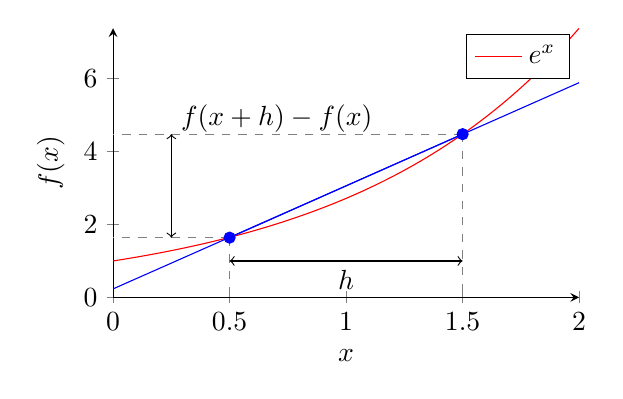
\begin{tikzpicture}
		\begin{axis}[
				axis lines = left,
				xlabel = \(x\),
				ylabel = {\(f(x)\)},
				width=7.5cm,
				height=5cm,
				xmin=0,
				ymin=0
			]

			\addplot [
				domain=0:2,
				samples=100,
				color=red,
			]
			{e^x};
			\addlegendentry{\(e^x\)}

			\addplot [
				domain=0:2,
				samples=100,
				color=blue,
			]
			{2.83*(x-0.5) + e^0.5};

			\addplot [
				color=blue,
				mark=*,
			]
			coordinates {
					(0.5, 1.64) (1.5,4.48)
				};

			\draw [dashed,gray] (axis cs:0.5,1.64) -- (axis cs:0.5,0);
			\draw [dashed,gray] (axis cs:1.5,4.48) -- (axis cs:1.5,0);
			\draw [dashed,gray] (axis cs:0.5,1.64) -- (axis cs:0,1.64);
			\draw [dashed,gray] (axis cs:1.5,4.48) -- (axis cs:0,4.48);

			\draw [<->] (axis cs:0.5,1) -- node [below]{\(h\)} (axis cs:1.5,1);
			\draw [<->] (axis cs:0.25,1.64) -- node [right,yshift=0.85cm]{\(f(x+h)-f(x)\)} (axis cs:0.25,4.48);
		\end{axis}
	\end{tikzpicture}
\end{wrapfigure}

\begin{definition}[Derivative]
	We can use the definitions of limits to define the derivative of a function \(f(x)\) with respect to its argument (in this case, \(x\)):
	\begin{equation}\label{derivative}
		\frac{\dd{f}}{\dd{x}} = \lim_{h \to 0} \frac{f(x+h)-f(x)}{h}
	\end{equation}
\end{definition}

Pictorially, we can see that the definition of the derivative is basically the slope of the line between two points that approach arbitrarily close to each other.
In this example, \(x\) is 0.5, and \(h\) is 1.

Note that for the derivative to exist at a point \(x\), we require that

\[
	\lim_{h \to 0^-} \frac{f(x+h)-f(x)}{h} = \lim_{h \to 0^+} \frac{f(x+h)-f(x)}{h}
\]

This excludes, for example, the derivative of \(\abs{x}\) at \(x=0\), as this would have two conflicting answers (\(-1\) and 1).

\subsection{Notation}
There are multiple ways of representing derivatives of functions.
Here, we show the derivative of \(f(x)\) in multiple notation systems:
\begin{itemize}
	\item \(\displaystyle \frac{\dd{f}}{\dd{x}}\): Leibniz notation
	\item \(f'(x)\): Lagrange notation
	\item \(\dot f (x)\): Newton notation
\end{itemize}

For sufficiently smooth functions (meaning that the derivative is valid at each step), we can define derivatives recursively:
\[
	\frac{\ddempty}{\dd{x}}\left( \frac{\dd{f}}{\dd{x}} \right)
	= \frac{\dn 2 f}{\dd{x}^2}
	= f''(x) = \ddot f (x)
\]

\subsection{Rules for Differentiation}
\begin{definition}[Chain Rule]
	Consider a function \(f(x) = F(g(x))\).
	The derivative of \(f(x)\) can be written
	\begin{equation}
		\frac{\dd{f}}{\dd{x}} = F'(g(x)) \cdot g'(x) = \frac{\dd{F}}{\dd{g}} \frac{\dd{g}}{\dd{x}}
	\end{equation}
\end{definition}

\begin{definition}[Product Rule]
	Consider a function \(f(x) = u(x)v(x)\).
	The derivative of \(f(x)\) can be written
	\begin{equation}
		\frac{\dd{f}}{\dd{x}} = u'(x)v(x) + u(x)v'(x) = u'v + uv'
	\end{equation}
\end{definition}

\begin{definition}[Leibniz' Rule]
	Consider a function \(f(x) = u(x)v(x)\).
	Recursive derivatives of \(f(x)\) can be written
	\begin{align}
		f    & = uv                                        \\
		f'   & = u'v + uv' \nonumber                       \\
		f''  & = u''v + 2u'v' + uv'' \nonumber             \\
		f''' & = u'''v + 3u''v' + 3u'v'' + uv''' \nonumber
	\end{align}
	This is analogous to Pascal's triangle and the binomial expansion.
	The coefficients are \(n!/m!(n-m)!
	\), more often written \(n \choose m\).
\end{definition}

\subsection{Order of Magnitude}
The goal of `order of magnitude' functions is to compare the size of functions in the vicinity of certain points.
\begin{definition}[Little \(o\)]
	Given functions \(f(x)\) and \(g(x)\) such that
	\begin{equation}
		\lim\limits_{x \to x_0} \frac{f(x)}{g(x)} = 0
	\end{equation}
	we can say that \(f(x) = o(g(x))\) as \(x \to x_0\).
\end{definition}

This is essentially saying that the function \(f(x)\) is much `smaller' than \(g(x)\) as we approach the point \(x_0\).
For example, \(x^2 = o(x)\) as \(x \to 0\), because \(x^2\) becomes vanishingly small compared to \(x\) near zero.

\begin{definition}[Big \(O\): \(x_0\) finite]
	Assume we have two functions \(f(x)\) and \(g(x)\), and a finite number \(x_0\) where we are comparing the functions.
	If we can find two positive constants \(M\) and \(\delta\) such that
	\begin{equation}
		\abs{f(x)} \leq M\abs{g(x)} \quad(\forall x,\, \abs{x-x_0} < \delta)
	\end{equation}
	then \(f(x) = O(g(x))\) as \(x \to x_0\).
\end{definition}
Informally, the function \(f\) can be \textit{bounded by} \(g\) in a specific area around the point \(x_0\).

Unlike little \(o\) notation, there is no requirement that \(f(x)\) becomes vanishingly small compared to \(g(x)\), just that it is smaller.
Therefore, \(x^2 \neq o(x^2)\) but \(x^2 = O(x^2)\) (both as \(x \to 0\)).

Some examples:
\begin{itemize}
	\item \(x^2 = O(x)\) as \(x \to 0\).
	      Take \(M = 1\), \(\delta = 1\).
	\item \(x \neq O(x^2)\) as \(x \to 0\).
	      This is because for any value of \(x\) smaller than \(1/M\), the value of \(g(x)\) is \(Mx^2\) which is smaller than \(x\).
	\item \(x^2 = O(x^2)\) as \(x \to 0\).
	      Take \(M = 1\), and choose an arbitrary \(\delta\).
\end{itemize}

By convention, we usually pick the most restrictive \(M\) and \(\delta\) possible.

\begin{definition}[Big \(O\): \(x_0\) infinite]
	Assume we have two functions \(f(x)\) and \(g(x)\), and we want to compare the functions' behaviours at infinity.
	If we can find two positive constants \(M\) and \(x_1\) such that
	\begin{equation}\label{bigoinf}
		\abs{f(x)} \leq M\abs{g(x)} \quad(\forall x > x_1)
	\end{equation}
	then \(f(x) = O(g(x))\) as \(x \to \infty\).
\end{definition}

This is basically the same as the previous definition --- but obviously we can't pick a value slightly less than infinity to test, so we just provide a lower bound on \(x\) where the condition holds true.

For example, \(2x^3 + 4x + 12 = O(x^3)\) as \(x \to \infty\).
This is because the function is a cubic, so can be bounded by a cubic as it shoots off to infinity.
We can take, for example, \(M = 3\) and \(x_1 = 3\).
Note that we can't just pick \(M=2\) even though asymptotically the function is close to \(2x^3\); there is a value added to the \(2x^3\) so we'd need to pick a slightly larger number to guarantee that Equation \eqref{bigoinf} is satisfied.

\subsection{Equation of a Tangent}
We can use little \(o\) notation to construct the equation of a tangent to a function \(f(x)\) at a given \(x\) value, \(x_0\).
This is the start of the formula for the Taylor series of \(f\) at \(x_0\).

First, notice that \(o(g(x))/g(x)\) is zero, as \(o(g(x))\) is vanishingly small compared to \(g(x)\) near the convergence point.

Using Equation \eqref{derivative}, we can (informally) deduce:

\begin{align*}
	\eval{\frac{\dd{f}}{\dd{x}}}_{x=x_0} & = \frac{f(x_0 + h) - f(x_0)}{h}                          \\
	                                     & = \frac{f(x_0 + h) - f(x_0)}{h} + \frac{o(h)}{h}         \\
	\therefore f(x_0 + h)                & = f(x_0) + \eval{\frac{\dd{f}}{\dd{x}}}_{x=x_0} h + o(h)
\end{align*}
If we now take \(x=x_0+h;\,y=f(x);\,y_0=f(x_0)\), we have
\[
	y = y_0 + \eval{\frac{\dd{f}}{\dd{x}}}_{x=x_0}(x - x_0) + o(h)
\]
This is the equation of the tangent to the curve at \(x_0\) if \(o(h)=0\), and this is start of the equation for the Taylor series.
